\section{Raytracing}
\subsection{Pixel Sampling}
As the raytracer is performing distribution raytracing each thread will perform multiple raytracing operations for each pixel
that it processes each sample per pixel is offset inside the pixel to perform antialiasing, this reduces the sharp edges that
can be seen in images. In order to improve the appearence of the image we also perform jittering on the samples this reduces
certain artifacts such as banding. \todo{Make sure the banding comment is correct and if so find a reference for it}

\missingfigure{anti-aliasing}

\subsection{Intersection Tests (0.5 pages)}
Intersection tests are another vital part of any raytracer. a number of intersection tests are needed, I will not include
an extensive treatment of the intersection tests mearly a listing of the most notable used.

\begin{description}
\item[Triangle] Moller-Trumbore intersection test \cite{MolTru97}
\item[AABB]
\item[kD-tree] As described in TODO:
\end{description}

\subsection{volume intersection}
Unlike intersection with all other object types the intersection with a participating media is non deterministic, this is
due to the fact that the intersection of the ray is determined by the extinction coefficient which gives a probablilty
of interaction, the depth of the interaction is calculated with equation \todo{add equation}, performing this non-deterministic
intersection test allows for objects within the medium to be interacted with when performing ray-marching.

\missingfigure{Non-deterministic intersection test}

\subsection{Intersection Storage}
When raytracing the scene the intersection point of the ray needs to be calculated and stored, this will include data that
is specific to an objects intersection, for example an intersection with a triangle mesh will need to record the trangle
that was intersected and as a result will need to record the barycentric coordinate at the point of intersection.

\subsection{Scene Traversal}

\section{Shading}

\subsection{Direct Illumination}
\subsubsection{Texture Mapping}
Performing texture mapping requires the ability to query the texture coordinates at a point of intersection, for mesh objects this
will interpolate the barycentric coordinates for the triangle of intersection, spheres use a spherical mapping that uses the
spherical coordinates to generate u,v values.

\subsection{Specular Reflection and Transmission}

\subsection{Nearest Neighbour Search}

\subsection{Diffuse Interreflection}
While it is possible to estimate the contribition to the radiance at an intersection point directly from the photon map this
approach can cause visual artifacts due to variance in the estimate in order to reduce these artifacts we perfom a final gather
stage at the point of intersect that produces a diffuse ray that is traced into the scene until a non-specular object is intesected,
we then perform the radiance at this point and use this information to estimate the radiance incident at the original point of intersection.
In order for the final gather to produce a correct estimate of the radiance we need to perform this stage multiple times per pixel, as we
are performing distributed raytracing this is a trivial addition. When calcualting the radiance for the final gather it has been shown \todo{cite}
that if the distance of the final gather point is lower than some threshold perfoming an additional diffuse bounce reduces errors at geometry
such as sharp corners where the radiance estimate can be inaccurate due to accounting for photons not truly at the surface.

\begin{figure}
\centering
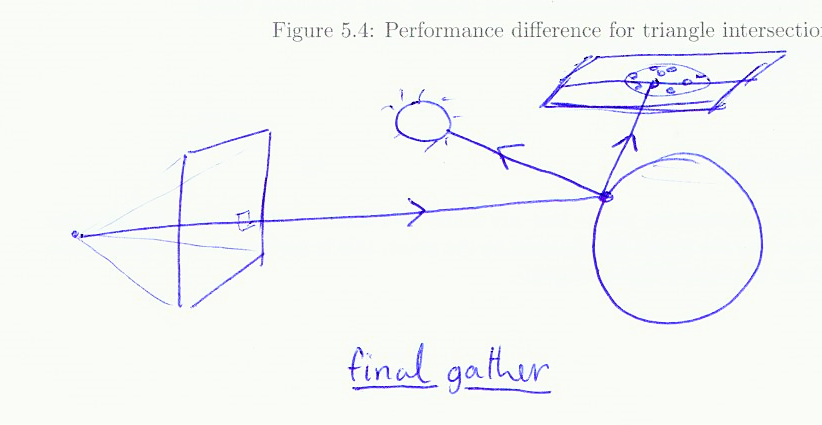
\includegraphics[width=\textwidth]{./images/final_gather.png}
\label{fig:final_gather}
\caption{Final Gather}
\end{figure}

\subsection{Caustics}

\subsection{Participating Media}

In the case of a ray that intersects a participating media before intersecting a surface we need to calculate three components to
the radiance along the path of the ray in the medium, these are single scattering direct illumination, multiple scattering (in-scattering)
and attenuation (out-scattering)

\subsubsection{Ray Marching}
In order to evaluate the radiace from the participating media we perform a ray-march, this is an iterative operation that evaluates the
radiance along the ray as it moves through the participating media.

\begin{equation}
L(x, \omega) = \sum\limits_{i = 1}^N L_l(x, \omega_l')p(x, \omega_l', \omega)\sigma_s(x)\Delta x + e^{- \sigma_t \Delta x} L (x + \omega \Delta x, \omega)
\end{equation}

\subsubsection{Attenuation}
As a ray travels through a medium the radiance can be reduced due to out-scattering and absortion, this can be calculated by evaluating
the integral given in equation \todo{Add the equation}, as we are only considering homogeneous participating media this can be
simplified as the properties being integrated are constant and a closed form solution is possible.

\missingfigure{Attenuation Equation}

\subsubsection{Direct Illumination}
At each point in the ray march we also evaluate the contribution from each light in the scene due to single scattering, this is performed
by performing an additional ray march in the direction of the light and evalute the radiance arriving at the point on the ray.

\subsubsection{Muliple Scattering}

